\documentclass{article}

%opening
\usepackage{graphbox}	% permette di modificare i margini
\usepackage{graphicx}
\usepackage{float}
\usepackage{longtable}
\usepackage{array}
\usepackage{fancyhdr}
\pagestyle{fancy}

\newcommand{\copertina}{
	\begin{titlepage}
		\begin{center}
			
			
\includegraphics[width=0.4\linewidth]{graphics/icon2.png}\\
			\vspace{1cm}
			
			\begin{Huge}
				\textbf{Centro Estetico Nirvana} \\
			\end{Huge}
			
			\vspace{9pt}  
			
			\begin{large}
				\textbf{Progetto per il concorso Accessibile Accattivante\\}
				\textbf{A.A.} 2022/2023\\
				\vspace{3pt}
			\end{large}	  
			
			\vspace{24pt}
			
			\begin{large}
				\textbf{Indirizzo sito web:} \href{http://tecweb.studenti.math.unipd.it/nbaesso}{http://tecweb.studenti.math.unipd.it/nbaesso}\\
			\end{large} 
			
			\begin{large}
				\textbf{Gruppo:} Accessibeauty\\
			\end{large} 

			\vspace{10pt} 
			
			\bgroup
			\def\arraystretch{1.3}
			\centering
			\begin{tabular}{r|L{5cm}}
			\multicolumn{2}{c}{\textbf{Informazioni sul gruppo} } \\ \hline
			\textbf{Membri} &  Nicola Baesso - 2011877 \newline Matteo Cusin - 2008073 \newline Annalisa Egidi - 1216745 \newline Lisien Skenderi - 2023461\\
			\end{tabular}
			\egroup
			
			\begin{center}
				\textbf{Referente\\}
				Nicola Baesso - nicola.baesso@studenti.unipd.it\\
				\textbf{Utenti (credenziali username-password):\\}
				\textit{Amministratore:} admin - admin\\
				\textit{Cliente:} user - user\\
			\end{center}
			
		\end{center}
	\end{titlepage}
}	%FINE NEW COMMAND COPERTINA

\usepackage{lastpage}
\usepackage{fancyhdr}
\fancypagestyle{plain}{
	% cancella tutti i campi di intestazione e piè di pagina
	\fancyhf{}
	
	\lhead{
		
\includegraphics[width=0.1\linewidth]{graphics/icon2.png}
	}
		\rhead{
		Centro Estetico Nirvana
	}

	\lfoot{ %piè di pagina a sx
		Concorso Accessibile Accattivante
	}
	\rfoot{Pagina \thepage{} di \pageref{LastPage}} %es: pag: 4 di 10
	
	%linea orizzontale alle posizioni top e bottom della pagina (se è 0, non c'è la linea)
	\renewcommand{\headrulewidth}{0.3pt}  
	\renewcommand{\footrulewidth}{0.3pt}
}
\pagestyle{plain}

\usepackage[utf8]{inputenc}
%\usepackage{cm-super}

\usepackage{lmodern}
\usepackage[T1]{fontenc}
\usepackage[italian]{babel} %il documento è in italiano
%\usepackage{textcomp} %The pack­age sup­ports the Text Com­pan­ion fonts, which pro­vide many text sym­bols
%(such as baht, bul­let, copy­right, mu­si­cal­note, onequar­ter, sec­tion, and yen), in the TS1 en­cod­ing.

\usepackage{graphicx}       %permette di inserire delle immagini
\usepackage{caption}        %numerazione figure e loro descrizione testuale
\usepackage{subcaption}     %sottofigure numerabili
\usepackage[dvipsnames,table]{xcolor}
\usepackage{rotating} %permette di ruotare le immagini

\usepackage{listings} %permette di inserire degli spezzoni di codice

\usepackage{tikz} %disegno di immagini vettoriali a schermo. Utile per grafi
\usetikzlibrary{arrows.meta}
\usetikzlibrary{graphs}
\usetikzlibrary{arrows}

%package per le tabelle
\usepackage{booktabs} %permette di poter usare delle liste nelle tabelle
\usepackage{tabularx} 
\usepackage{longtable} %una tabella può continuare su più pagine
\usepackage{multirow} %utile per visualizzare una cella su più righe

%crea una cella per le tabelle in grado di andare a capo con \newline
%https://tex.stackexchange.com/questions/12703/how-to-create-fixed-width-table-columns-with-text-raggedright-centered-raggedlef
\usepackage{array}
\newcolumntype{L}[1]{>{\raggedright\let\newline\\\arraybackslash\hspace{0pt}}m{#1}}
\newcolumntype{C}[1]{>{\centering\let\newline\\\arraybackslash\hspace{0pt}}m{#1}}
\newcolumntype{R}[1]{>{\raggedleft\let\newline\\\arraybackslash\hspace{0pt}}m{#1}}


%indice con i puntini
\usepackage{tocloft}
\renewcommand\cftsecleader{\cftdotfill{\cftdotsep}}

%http://ctan.mirror.garr.it/mirrors/CTAN/macros/latex/contrib/appendix/appendix.pdf
\usepackage{appendix} %aggiunge dei comandi per l'appendice
\usepackage{parskip} %aiuta LaTeX a trovare il miglior stile per i page break
\setcounter{secnumdepth}{5} % numera i sottoparagrafi
\setcounter{tocdepth}{5} %aggiunge all'indice i sottoparagrafi
%\usepackage{titlesec} %\begin{paragraph} si può usare come subsubsubsection!

\usepackage{breakurl}%\url{...} può continare alla linea successiva. (si può andare a capo)

\usepackage[colorlinks=true]{hyperref}
\hypersetup{
	colorlinks=true,
	citecolor=black,
	filecolor=black,
	linkcolor=black, % colore dei link interni
	urlcolor=Maroon  % colore dei link interniesterni
}

%per alcune liste, permette di usare 'alligator' nei labeling 
\usepackage{blindtext} 
\usepackage{scrextend} 
\addtokomafont{labelinglabel} 
{\sffamily}

%FILE INCLUSI
\usepackage{graphicx}

\begin{document}

\copertina
\tableofcontents
\newpage
\section{Introduzione}
Il sito proposto per il concorso riguarda il centro estetico Nirvana, che desidera implementare un sito Internet al fine di poter fornire informazioni riguardo al centro stesso.\\
Il sito contiene informazioni sui trattamenti disponibili e sui macchinari utilizzati per essi, nonchè informazioni sulle consulenze e ogni informazione relativa alla locazione del centro e quali orari di apertura osserva.\\
Inoltre, permette agli utenti di richiedere una consulenza o un trattamento, che necessita di essere confermato o meno dal centro stesso. Le prenotazioni possono anche essere inserite dai dipendenti del centro stesso.\\
É fondamentale che il sito garantisca accessibilitá, in modo da permettere a chiunque di poter essere utilizzato, e usabilitá, separando struttura, presentazione e comportamento.\\
Si vuole infine garantire una navigazione fluida tra i contenuti del sito, evitando al piú possibile il disorientamento e prevedendo il giusto supporto per ritornare all'interno del sito stesso.
\section{Fase di Test}
Come per ogni prodotto software, anche per i siti web é necessario stabilire dei test in modo da verificare la funzionalitá di un sito.\\
A maggior ragione, bisogna assicurarsi che il sito sia fruibile da piú dispositivi possibili e in piú modalitá possiibili.\\
Ovviamente questo progetto non fa eccezione, e per tale scopo si sono create le seguenti macro-aree di test:
\begin{itemize}
	\item Browser Desktop: verificare che browser come Chrome, Firefox, Safari e Opera permettano l'utilizzo del sito senza problematiche a livello grafico o comportamentale;
	\item Browser Mobile: verificare che il sito sia fruibile mediante uno smartphone o un dispositivo mobile;
	\item Screen Readers: verificare che il sito sia fruibile anche senza guardarlo (!), solamente "ascoltando" le informazioni che il sito stesso rivela;
	\item Navigazione da tastiera: verificare che i contenuti possano essere utilizzati anche solo con la tastiera (ció si include, almeno in parte, con l'utilizzo di uno screen reader)
\end{itemize}
Nella prossima sezione vengono elencati gli strumenti utilizzati per garantire le funzionalitá descritte.
%nuova sezione
\section{Strumenti}
Essendo lo scopo del progetto lo sviluppo di un sito web che possa essere utilizzato da qualunque tipologia di utente e con qualunque disabilitá (visiva o motoria), é stato necessario utilizzare degli strumenti per controllare l'efficacia della navigazione nel sito stesso.\\
Vengono sottolineate due categorie di strumenti poiché alcuni strumenti utilizzati non sono adatti per una fase di test, ma risultano estremamente utili come aiuto allo sviluppo.
\subsection{Strumenti di sviluppo}
\subsubsection*{Silktide}
Silktide, sviluppato dall'omonima azienda, é un'estensione per browser che permette di simulare diverse disabilitá, come:
\begin{itemize}
	\item Dislessia
	\item Discromatopsia
	\item Miopia
	\item Perdita di visione periferica o centrale
	\item Cecitá totale
\end{itemize}
In particolare, integra uno screen reader per simulare la cecitá totale, utile per identificare bottoni o elementi senza descrizione.\\
Sebbene non possa sostituire uno screen reader reale come NVDA o OCRA, é risultato interessante il suo utilizzo specie per lo sviluppo di avvisi indipendenti dal colore.
\begin{figure}[H]
	\centering
	\fbox{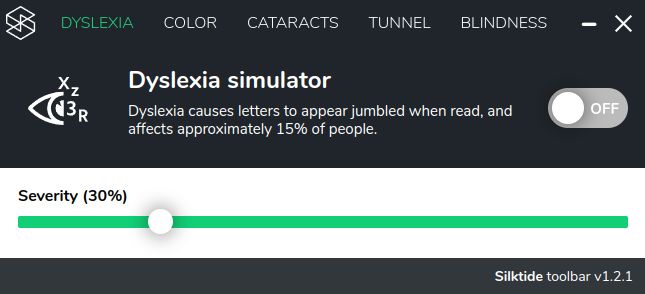
\includegraphics[scale=0.69]{./graphics/silktide.png}}
	\caption{Schermata iniziale di Silktide}
\end{figure}
\subsection{Strumenti di test}
\subsubsection*{NVDA}
NVDA, acronimo di NonVisual Desktop Access, è uno screen reader sviluppato per Windows.\\
Essendo gratuito, risulta largamente piú diffuso di screen readers come JAWS (a pagamento) o OCRA (disponibile gratuitamente su Linux).\\
É quindi sembrato il candidato ideale per testare la navigazione del sito da parte di un utente con disabilitá visive estremamente importanti.
\begin{figure}[H]
	\centering
	\fbox{
\includegraphics[scale=0.65]{./graphics/nvda.png}}
	\caption{Logo di NVDA}
\end{figure}
\subsubsection*{Links}
Links è un browser open source testuale con interfaccia a riga di comando.\\
Disponendo di una semplice interfaccia grafica da terminale, può visualizzare pagine complesse (ha supporto all'HTML 4.0 parziale con tabelle e frame, supporto per molteplici set di caratteri), supporta terminali a colori e monocromatici, e permette lo scrolling orizzontale.\\
Le sue caratteristiche sono risultate perfette per controllare che la navigazione del sito non fosse legata alla parte grafica o al comportamento, ma solamente alla struttura del sito stesso.

\begin{figure}[H]
	\centering
	\fbox{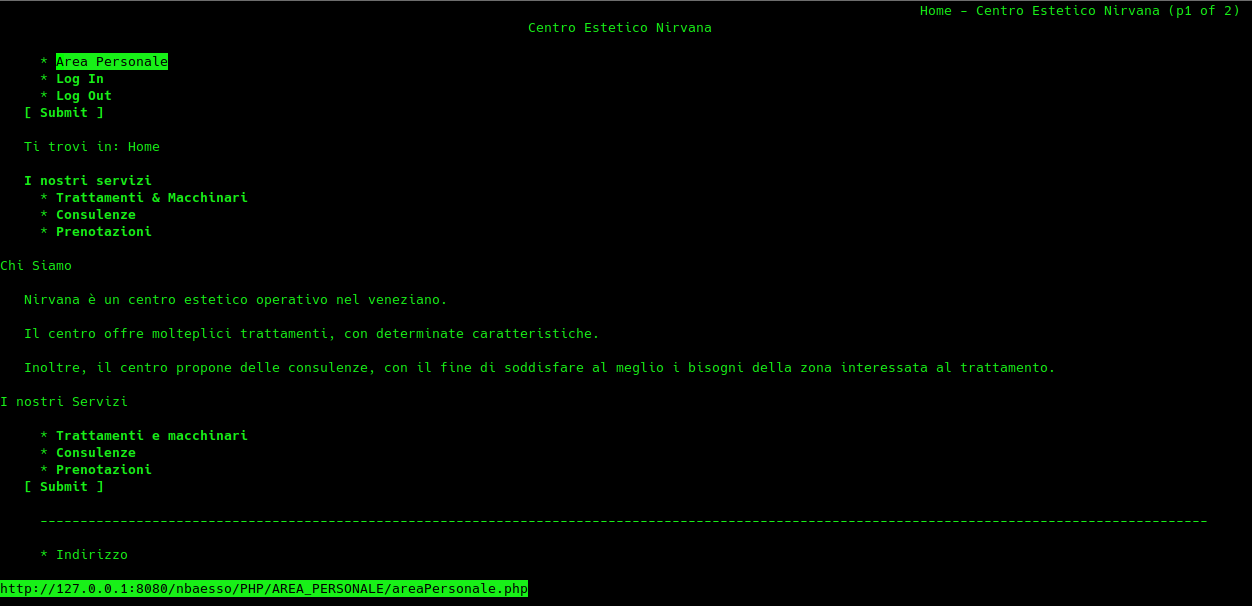
\includegraphics[scale=0.35]{./graphics/links.png}}
	\caption{Pagina principale del sito vista da Links}
\end{figure}
\end{document}
